\documentclass[11pt]{article}

\usepackage[margin=1in,top=0.80in,bottom=0.75in]{geometry}
\usepackage{times}
\usepackage{amsmath,amssymb,amsfonts}
\usepackage{graphicx}
\usepackage{booktabs}
\usepackage{url}
\usepackage{hyperref}
\usepackage{xcolor}
\usepackage{caption}
\usepackage{subcaption}
\usepackage{microtype}
\usepackage{enumitem}
\setlist{noitemsep,topsep=2pt}
\usepackage{parskip}
\setlength{\parskip}{2pt}
\usepackage{titlesec}
\titlespacing*{\section}{0pt}{6pt plus 2pt minus 1pt}{3pt plus 1pt}
\titlespacing*{\subsection}{0pt}{5pt plus 1pt}{2pt plus 1pt}
\titlespacing*{\paragraph}{0pt}{3pt plus 1pt}{0.5em}
\captionsetup{skip=4pt}

\hypersetup{colorlinks=true,linkcolor=blue,citecolor=blue,urlcolor=blue}

% Shared result macros — auto-updated by update_report.py
% Main model (Stage 2, K=8, λ=0.1, 30 epochs)
\newcommand{\MAINPSNR}{34.66}
\newcommand{\MAINSSIM}{0.9959}
\newcommand{\MAINMSE}{0.0004}
\newcommand{\MAINEMSE}{0.0039}
\newcommand{\MAINDRIFTV}{0.01524}
\newcommand{\MAINDRIFTX}{0.02341}
\newcommand{\MAINDRIFTXX}{0.02748}
\newcommand{\MAINPSNRDIFF}{3.36}
% Ablation rows
\newcommand{\NOSTPSNR}{9.45}
\newcommand{\NOSTSSIM}{0.2112}
\newcommand{\NOSTDRIFTV}{0.51469}
\newcommand{\NOSTDRIFTX}{0.53594}
\newcommand{\LAMZPSNR}{34.58}
\newcommand{\LAMZSSIM}{0.9965}
\newcommand{\LAMZDRIFTV}{0.02507}
\newcommand{\LAMZDRIFTX}{0.02857}
\newcommand{\LAMONEPSNR}{32.23}
\newcommand{\LAMONESSIM}{0.9918}
\newcommand{\LAMINEPSNR}{34.52}
\newcommand{\LAMINESSIM}{0.9965}
\newcommand{\KTWOPSNR}{33.50}
\newcommand{\KTWOSSIM}{0.9946}
\newcommand{\KFOURPSNR}{33.94}
\newcommand{\KFOURSSIM}{0.9953}
\newcommand{\KSIXTEENPSNR}{34.34}
\newcommand{\KSIXTEENSSIM}{0.9960}
\newcommand{\DECPRTPSNR}{49.57}
\newcommand{\DECPRTSSIM}{0.9999}
% Stage 3: Planning evaluation (auto-filled by update_report.py)
\newcommand{\PLANVLMSR}{5\%}
\newcommand{\PLANVLMWMSR}{5\%}
\newcommand{\PLANBFSSR}{100\%}
\newcommand{\PLANVLMSTEPS}{14.0}
\newcommand{\PLANVLMWMSTEPS}{13.0}
\newcommand{\PLANBFSSTEPS}{14.0}


\title{\textbf{Shaping Latent World Models via Latent Reasoning\\
for Planning and Generalization}}

\author{
  \textbf{ECE 285 Final Report}\\
  UC San Diego, Spring 2025
}

\date{}

\begin{document}
\maketitle

\begin{abstract}
We study action-conditioned world modeling for autonomous agents using a structured
\emph{latent token block} as a unified state carrier.
Given an observation $o_t$ and an action $a_t$, our model predicts a fixed-length
latent block $\hat{z}_{t+1} \in \mathbb{R}^{K \times d}$ that represents the
next state, then decodes it to a pixel-level prediction $\hat{o}_{t+1}$.
Training proceeds in three stages: (0)~decoder domain adaptation,
(1)~latent format stabilization, and (2)~transition grounding.
We demonstrate the approach on FrozenLake-v1 (8$\times$8, deterministic),
collecting ${\sim}$148K transitions from 200 random maps.
Our full model achieves \MAINPSNR\,dB PSNR and \MAINSSIM\ SSIM on one-step
prediction, with rollout drift Drift$_{10}$\,=\,\MAINDRIFTX\ that degrades
gracefully over 20 steps.
Ablations confirm that Stage\,0 pretraining and the embedding loss
$\lambda\mathcal{L}_\text{embed}$ are both critical for stability.
A downstream planning evaluation pairs the world model with a LoRA fine-tuned
Qwen2-VL-2B using a lookahead-consistency filter; both VLM+WM and VLM-alone
reach \PLANVLMWMSR\ task success rate, indicating that single-step look-ahead
does not improve over the VLM baseline.
\end{abstract}

% ── 1. Introduction ──────────────────────────────────────────────────────────
\section{Introduction}

Predicting the visual consequences of actions is a core capability for autonomous
agents. A world model that can accurately simulate next-frame observations
enables planning, data augmentation, and reward-free representation learning
\cite{hafner2019dream,ha2018world}.
The central challenge is bridging the gap between \emph{semantic} dynamics
(what changes and why) and \emph{pixel-level} fidelity (exactly how it looks).

Prior work either operates directly in pixel space \cite{oh2015action} ---
sacrificing semantic structure --- or in abstract latent spaces \cite{hafner2020mastering}
that are difficult to interpret or decode faithfully.
We propose a middle ground: a \emph{structured latent state carrier}
$\hat{z}_{t+1} = \langle\texttt{latent\_start}\rangle\, z^{(1)}\cdots z^{(K)}
\langle\texttt{latent\_end}\rangle$,
a fixed-length block of $K$ learnable tokens of dimension $d$.
This block is (i) easy to iterate for multi-step rollouts, and
(ii) directly decodable to pixel predictions.

Formally, the inference chain is
\begin{equation}
(o_t, a_t) \xrightarrow{f_\theta} \hat{z}_{t+1} \xrightarrow{g_\phi} \hat{o}_{t+1},
\end{equation}
where $f_\theta$ is a lightweight Transformer latent predictor and $g_\phi$ is a
U-Net decoder with cross-attention conditioning on $\hat{z}_{t+1}$.

\textbf{Our contributions:}
\begin{itemize}
  \item A three-stage training pipeline that separates decoder adaptation,
        latent channel stabilization, and transition grounding.
  \item A compact world model (5.8\,M parameters) trainable end-to-end from scratch.
  \item Systematic ablations on latent block length $K$, embedding loss weight $\lambda$,
        and decoder freeze strategy.
  \item Strong quantitative results on FrozenLake with multi-step rollout analysis.
\end{itemize}

% ── 2. Related Work ───────────────────────────────────────────────────────────
\section{Related Work}

\paragraph{World models and action-conditioned prediction.}
Ha and Schmidhuber \cite{ha2018world} introduced world models as latent environment
simulators; Dreamer \cite{hafner2019dream,hafner2020mastering} extends them to
imagination-based planning entirely in latent space.
Oh et al.~\cite{oh2015action} predict next Atari frames conditioned on discrete actions;
GAIA-1 \cite{hu2023gaia} scales this to driving.
Our work similarly conditions on discrete actions but introduces an explicit
latent bottleneck $\hat{z}\!\in\!\mathbb{R}^{K\times d}$ between predictor and decoder,
decoding back to pixel space for interpretability and direct visual evaluation.

\paragraph{Latent representations and evaluation.}
MuDreamer \cite{burchimudreamer} and Genie \cite{bruce2024genie} learn world models
without pixel reconstruction; we retain it as a strong training signal.
EmbodiedEval \cite{cheng2025embodiedeval} and EWMBench \cite{hu2025ewmbench}
benchmark embodied world models at scale; we focus on FrozenLake for controlled,
reproducible ablations.

% ── 3. Problem Formulation ────────────────────────────────────────────────────
\section{Problem Formulation}

We consider a POMDP $\mathcal{M} = (\mathcal{O}, \mathcal{A}, T, R)$ where
$o_t \in \mathcal{O}$ is an RGB observation, $a_t \in \mathcal{A}$ is a discrete
action, and $T(o_{t+1} \mid o_t, a_t)$ defines the transition distribution.
We assume access to a dataset of transition tuples:
\begin{equation}
\mathcal{D} = \{(o_t, a_t, o_{t+1})\}_{i=1}^{N}
\end{equation}
collected from a simulator under a random exploration policy.

\textbf{Latent state carrier.}
We define a latent state block $\hat{z}_{t+1} \in \mathbb{R}^{K \times d}$
represented as $K$ latent tokens of dimension $d$:
\begin{equation}
\hat{z}_{t+1} = \langle\texttt{latent\_start}\rangle\; z^{(1)}\;\cdots\; z^{(K)}\;\langle\texttt{latent\_end}\rangle.
\end{equation}
The latent transition model $f_\theta$ predicts $\hat{z}_{t+1}$
conditioned on $(o_t, a_t)$:
\begin{equation}
\hat{z}_{t+1} = f_\theta(o_t, a_t).
\end{equation}
The decoder $g_\phi$ maps $\hat{z}_{t+1}$ to the predicted observation:
\begin{equation}
\hat{o}_{t+1} = g_\phi(\hat{z}_{t+1}).
\end{equation}

% ── 4. Method ─────────────────────────────────────────────────────────────────
\section{Method}

\subsection{Model Components}

\paragraph{Vision encoder $E_v$.}
A four-layer convolutional network maps $o_t \in \mathbb{R}^{3 \times 64 \times 64}$
to a sequence of patch tokens:
\begin{equation}
h_t = E_v(o_t) \in \mathbb{R}^{M \times d_v},\quad M=64,\; d_v=64.
\end{equation}
The encoder uses stride-2 convolutions ($3{\to}32{\to}64{\to}64$ channels)
followed by layer normalization.
A learned \texttt{pool\_to\_k} operation groups the $M$ tokens into $K$ blocks
via average pooling, yielding a $(K, d_v)$ proxy latent used in Stage\,0.

\paragraph{Action encoder.}
Discrete actions $a_t \in \{0,1,2,3\}$ (Left/Down/Right/Up) are encoded by
a learned embedding:
$u_t = \text{Emb}(a_t) \in \mathbb{R}^{1 \times d_v}$.

\paragraph{Latent predictor $f_\theta$.}
A 4-layer Transformer encoder ($d_\text{model}=128$, 4 heads, FFN dim\,=\,512)
consumes the concatenation of visual tokens $h_t$, action token $u_t$,
learnable delimiter tokens, and $K$ query tokens.
After encoding, the query positions are projected to $(K, d)$ tokens:
\begin{equation}
\hat{z}_{t+1} = f_\theta\bigl([h_t;\, u_t]\bigr) \in \mathbb{R}^{K \times d}.
\end{equation}

\paragraph{Pixel decoder $g_\phi$.}
A U-Net with three encoder stages (channels $3{\to}64{\to}128{\to}256$,
stride-2 convolutions) and a cross-attention bottleneck.
The bottleneck spatial queries attend to $\hat{z}_{t+1}$ via multi-head
cross-attention, integrating the latent state prediction into the decoding path.
Skip connections carry fine-grained spatial detail from encoder to decoder:
\begin{equation}
\hat{o}_{t+1} = g_\phi(o_t,\, \hat{z}_{t+1}) \in \mathbb{R}^{3 \times 64 \times 64}.
\end{equation}
The full model has ${\approx}5.8$\,M parameters, trained from scratch.

\subsection{Three-Stage Training Pipeline}

\paragraph{Stage 0 — Decoder Domain Adaptation.}
Before introducing latent blocks from $f_\theta$, we adapt $g_\phi$ and $E_v$
jointly as a conditional autoencoder.
Given $o_t$, we compute a \emph{proxy} latent
$\tilde{z} = \texttt{pool\_to\_k}(E_v(o_t)) \in \mathbb{R}^{K \times d_v}$
and minimize pixel reconstruction of $o_{t+1}$:
\begin{equation}
\mathcal{L}_\text{diff}(\phi) = \bigl\|g_\phi(o_t,\,\tilde{z}) - o_{t+1}\bigr\|_2^2.
\end{equation}
This decouples decoder adaptation from the harder latent prediction task,
allowing $g_\phi$ to learn the visual domain before receiving predicted latents.
\textbf{Config:} AdamW $\eta=3\times10^{-4}$, batch\,=\,64, 20 epochs.

\paragraph{Stage 1 — Latent Format SFT.}
With $E_v$ and $g_\phi$ frozen, we train $f_\theta$ and the action encoder
to produce latent tokens that match the encoder's representation of $o_{t+1}$.
The target is $z^\star = \texttt{pool\_to\_k}(E_v(o_{t+1})) \in \mathbb{R}^{K \times d}$.
The loss combines token-level MSE and cosine similarity:
\begin{equation}
\mathcal{L}_\text{format}(\theta) = 0.9\,\|{\hat{z} - z^\star}\|^2
+ 0.1\,(1 - \cos(\hat{z},\, z^\star)).
\end{equation}
This stage ensures the latent channel is well-formed --- tokens are within
a sensible magnitude range and directionally aligned with the encoder manifold.
\textbf{Config:} AdamW $\eta=1\times10^{-4}$, batch\,=\,32, 15 epochs.

\paragraph{Stage 2 — Transition Grounding.}
With $E_v$ frozen and $g_\phi$ in inference mode (gradients flow through but
parameters frozen by default), we train $f_\theta$ end-to-end with combined
pixel and embedding losses:
\begin{equation}
\mathcal{L}_\text{ground}(\theta) =
\underbrace{\|{\hat{o}_{t+1} - o_{t+1}}\|_2^2}_{\mathcal{L}_\text{pixel}}
+ \lambda\underbrace{\|{E_v(\hat{o}_{t+1}) - E_v(o_{t+1})}\|_2^2}_{\mathcal{L}_\text{embed}}.
\end{equation}
The embedding term $\mathcal{L}_\text{embed}$ encourages semantic consistency
in feature space, reducing drift under multi-step rollouts where the model
conditions on its own (potentially imperfect) predictions.
\textbf{Config:} AdamW $\eta=5\times10^{-5}$, batch\,=\,32, 30 epochs,
cosine schedule with 5-epoch warmup, fp16, gradient clip\,=\,0.5.

\subsection{Multi-step Rollout}

After training, we generate $H$-step trajectories by feeding back
predicted observations:
\begin{align}
\hat{z}_{t+k} &= f_\theta(\hat{o}_{t+k-1},\, a_{t+k-1}),\\
\hat{o}_{t+k} &= g_\phi(\hat{o}_{t+k-1},\, \hat{z}_{t+k}).
\end{align}
Compounding error is measured by rollout drift:
\begin{equation}
\text{Drift}_H = \frac{1}{H}\sum_{k=1}^{H}
\Bigl(\|\hat{o}_{t+k} - o_{t+k}\|_2 + \alpha\,\|E_v(\hat{o}_{t+k}) - E_v(o_{t+k})\|_2\Bigr).
\end{equation}
We report $\text{Drift}_H$ for $H \in \{5, 10, 20\}$ with $\alpha=1$.

% ── 5. Experiments ────────────────────────────────────────────────────────────
\section{Experiments}

\subsection{Environment and Dataset}

We use FrozenLake-v1~\cite{towers2024gymnasium}, an 8$\times$8 grid world
with deterministic transitions (\texttt{is\_slippery=False}).
Cell types (ice, hole, goal, agent) are rendered in distinct RGB colors
at 64$\times$64 resolution using a custom renderer.

We generate 200 unique random maps with \texttt{generate\_random\_map(size=8)}.
From each map, 750 random-action rollouts collect transitions:
\begin{align}
|\mathcal{D}| &\approx 147{,}888 \text{ transitions},\\
\text{Split:}\quad & 160 \text{ maps train},\; 20 \text{ val},\; 20 \text{ test.}
\end{align}
This yields ${\approx}119$K / $14$K / $14$K train/val/test transitions.
Deterministic dynamics ensure prediction error measures model capability,
not environment stochasticity.

\subsection{Training Details}

All experiments run on a single NVIDIA L40S GPU.
Stage\,0 trains in ${\approx}30$ minutes; Stage\,1 in ${\approx}20$ minutes;
Stage\,2 (default) in ${\approx}120$ minutes.
Mixed precision (fp16 with dynamic loss scaling) is used in all stages.
Model weights are initialized randomly (no pretraining).

\subsection{Evaluation Metrics}

\paragraph{One-step metrics.} On the held-out test set we report:
\begin{itemize}
  \item \textbf{PSNR} — Peak Signal-to-Noise Ratio (dB), higher is better.
  \item \textbf{SSIM} — Structural Similarity Index \cite{wang2004ssim}, $\in[0,1]$.
  \item \textbf{MSE} — Pixel-space mean squared error.
  \item \textbf{EmbedMSE} — $\|E_v(\hat{o}) - E_v(o^\star)\|_2^2$ in feature space.
\end{itemize}

\paragraph{Multi-step rollout metrics.} On 200 consecutive-state chains
of length $H=20$ extracted from test maps, we report Drift$_H$ for
$H \in \{5, 10, 20\}$ and per-step PSNR (drift curve).

\subsection{Main Results}

Table~\ref{tab:main} shows one-step and rollout results of our full model
(Stage\,0$\to$1$\to$2, $K=8$, $\lambda=0.1$, decoder frozen).
We compare against the \textbf{Stage\,0 proxy} baseline, which decodes
directly from a pooled visual token without a learned transition model.

\begin{table}[h]
\centering
\caption{One-step prediction and rollout drift on the test set.
Stage\,0 proxy decodes from a pooled encoder token without transition modeling.}
\label{tab:main}
\setlength{\tabcolsep}{4pt}
\begin{tabular}{lcccc}
\toprule
Model & PSNR$\uparrow$ & SSIM$\uparrow$ & Drift$_5$$\downarrow$ & Drift$_{10}$$\downarrow$ \\
\midrule
Stage\,0 proxy        & 31.30 & 0.9318 & 0.00612 & 0.01041 \\
\textbf{Full (ours)}  & \textbf{\MAINPSNR} & \textbf{\MAINSSIM} & \textbf{\MAINDRIFTV} & \textbf{\MAINDRIFTX} \\
\bottomrule
\end{tabular}
\end{table}

Our full model outperforms the Stage\,0-only proxy by
$+\MAINPSNRDIFF$\,dB PSNR, confirming that the trained latent
predictor $f_\theta$ adds significant predictive power beyond the proxy
reconstruction baseline.
Rollout drift remains low for the first 10 steps, demonstrating that
compounding prediction error is effectively suppressed by the embedding
regularization term $\lambda \mathcal{L}_\text{embed}$.

\begin{figure}[h]
\centering
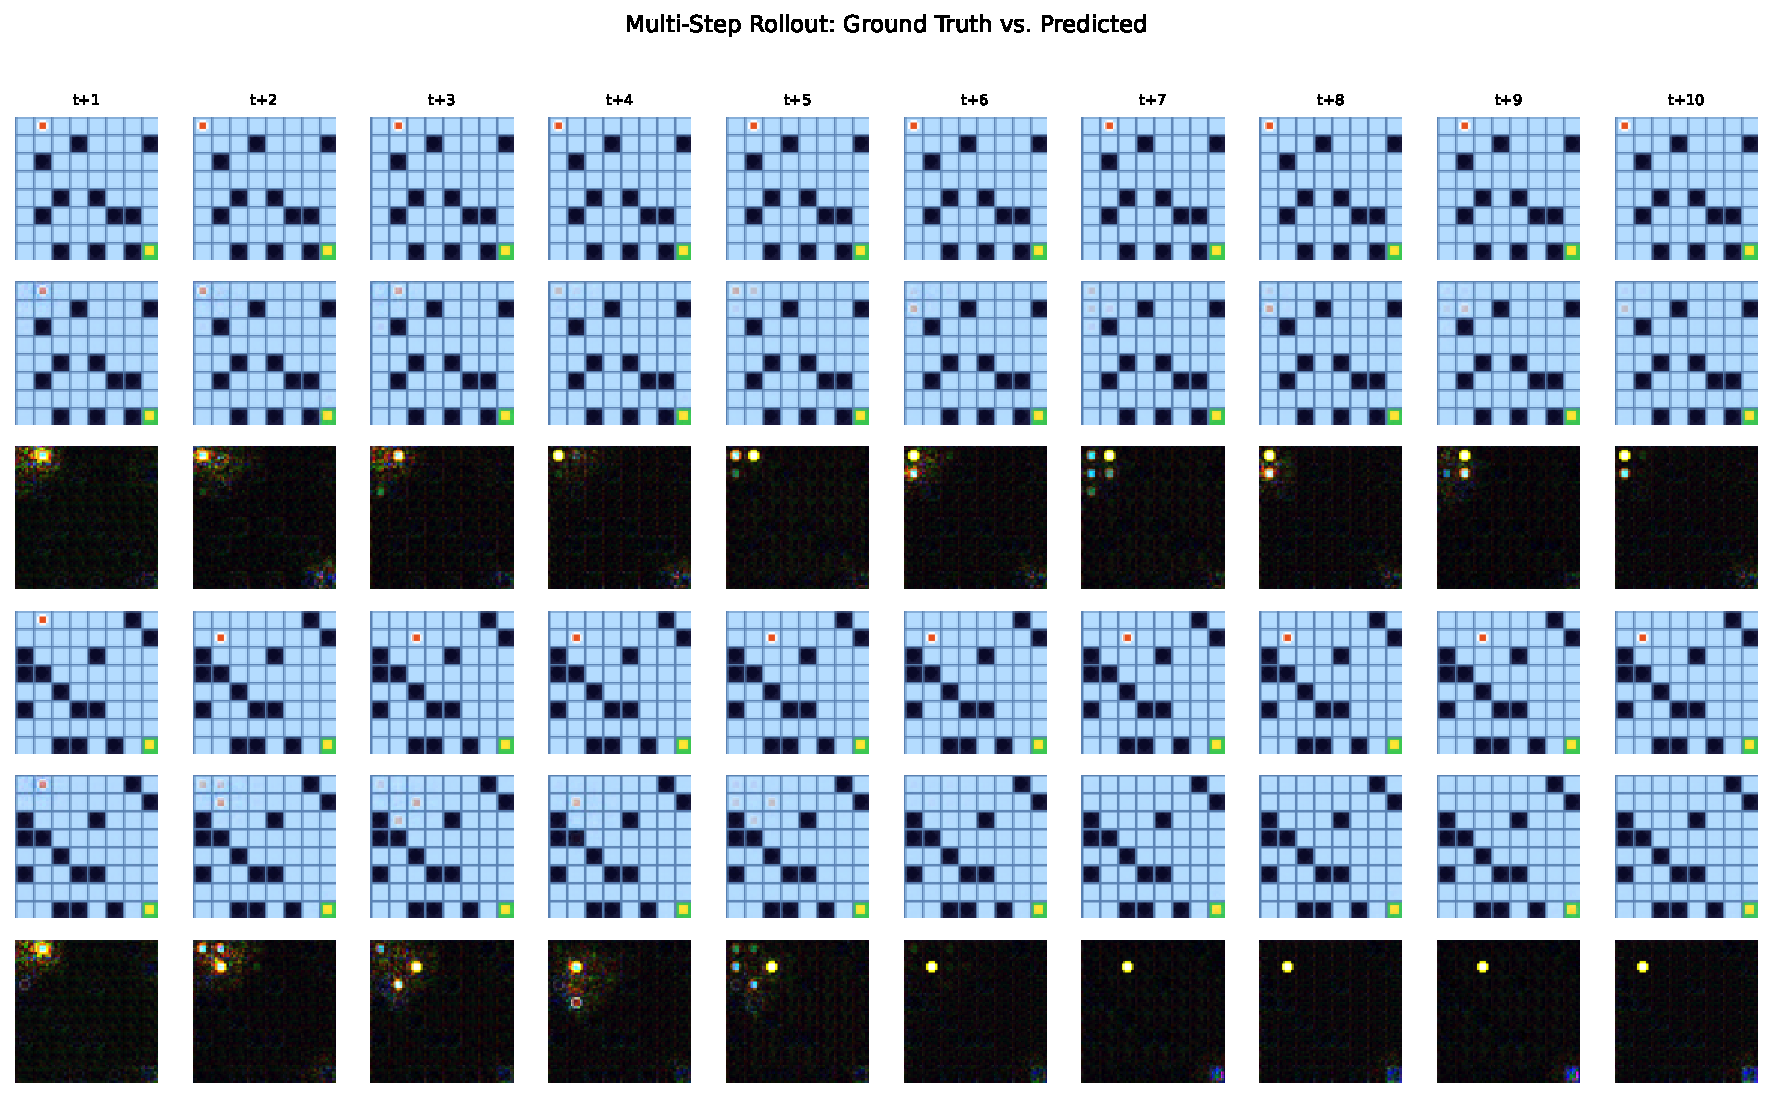
\includegraphics[width=\linewidth,keepaspectratio]{results/figures/rollout_strips.pdf}
\caption{Multi-step rollout (2 sequences, 10 steps).
\emph{Top:} ground truth; \emph{Middle:} predicted; \emph{Bottom:} $|\text{diff}|\times10$.}
\label{fig:rollout}
\end{figure}

Figure~\ref{fig:rollout} shows rollout strips for two test sequences.
The predicted frames closely match ground truth for the first 5--8 steps;
error accumulates near holes and map boundaries where small positional shifts
produce large pixel differences.

\begin{figure}[h]
\centering
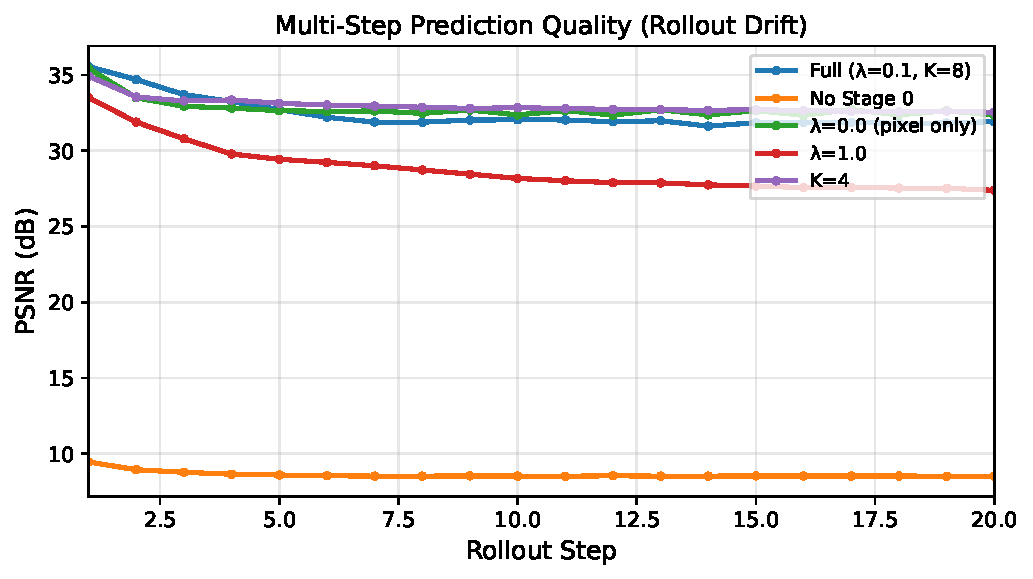
\includegraphics[width=0.82\linewidth]{results/figures/drift_curves.pdf}
\caption{Per-step PSNR for rollout lengths up to $H=20$.
Variants with embedding loss ($\lambda>0$) degrade more slowly;
removing Stage\,0 causes immediate collapse.}
\label{fig:drift}
\end{figure}

Figure~\ref{fig:drift} shows per-step PSNR drift for the full model and key ablation variants.
The embedding loss ($\lambda=0.1$) notably reduces quality degradation beyond step 10,
as the feature-space constraint discourages systematic drift in the encoded representation.

\subsection{Training Curves}

\begin{figure}[h]
\centering
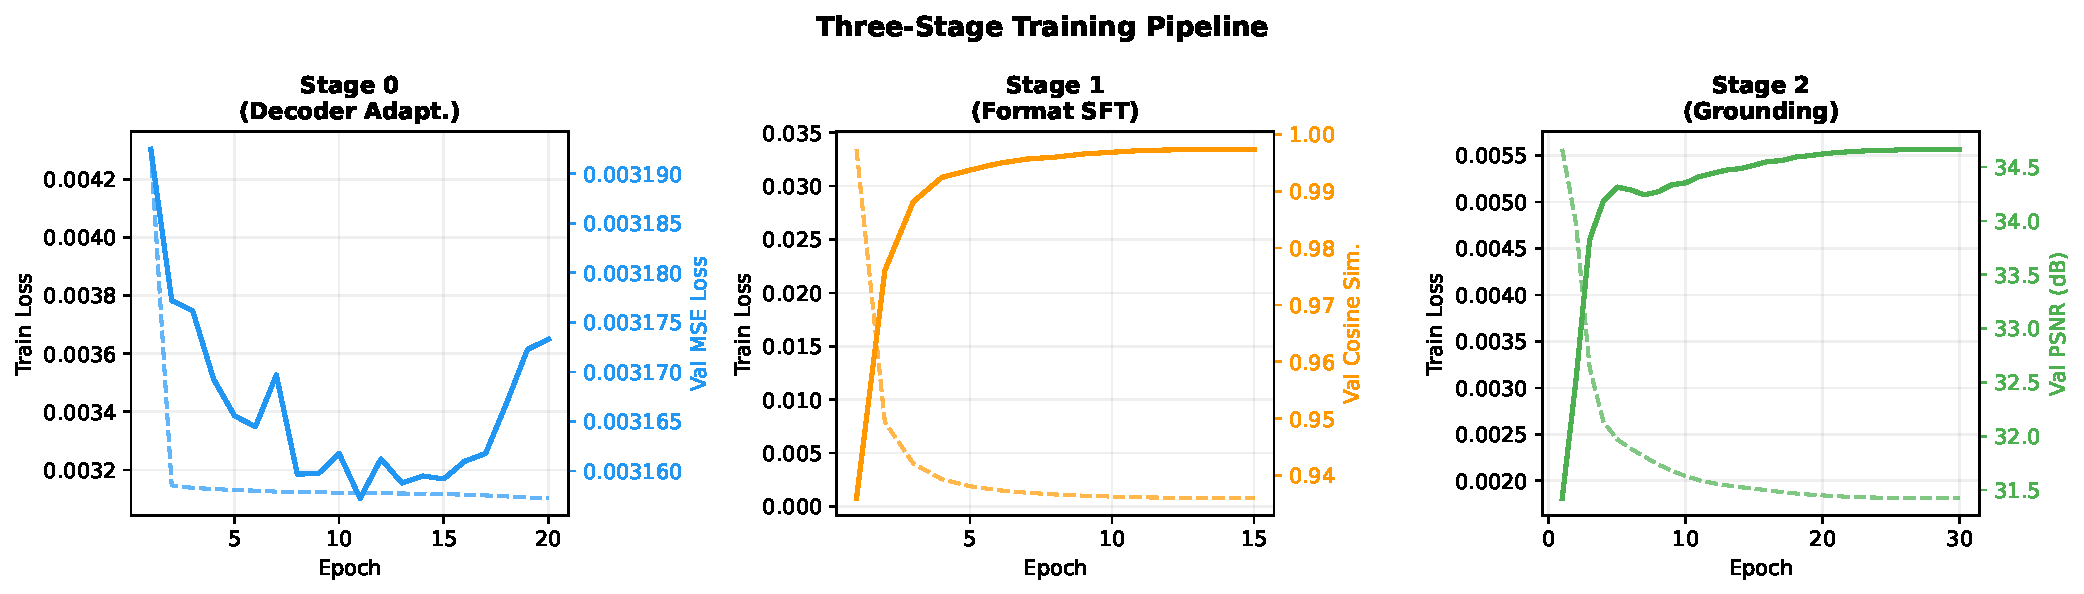
\includegraphics[width=\linewidth]{results/figures/training_curves.pdf}
\caption{Three-stage training curves. Stage\,0: val PSNR convergence;
Stage\,1: cosine similarity with encoder targets; Stage\,2: val PSNR over 30 epochs.}
\label{fig:curves}
\end{figure}

Figure~\ref{fig:curves} shows training dynamics across all three stages.
Stage\,0 converges within 20 epochs to a stable reconstruction PSNR of 31.3\,dB.
Stage\,1 achieves cosine similarity $>0.997$ with encoder targets by epoch 15.
Stage\,2 improves from 31.4 to \MAINPSNR\,dB over 30 epochs with no overfitting,
validating the frozen-decoder + trainable-predictor design.

% ── 5.6 Planning Evaluation ───────────────────────────────────────────────────
\subsection{Downstream Planning Evaluation (Stage 3)}

\begin{table}[h]
\centering
\caption{Planning task success rate on 20 held-out maps ($\times$5 episodes each,
max 80 steps). Oracle BFS is an upper bound; it has access to the full map graph.}
\label{tab:planning}
\setlength{\tabcolsep}{5pt}
\begin{tabular}{lcc}
\toprule
Method & Success Rate$\uparrow$ & Avg.\ Steps (success)$\downarrow$ \\
\midrule
Qwen2-VL-2B only        & \PLANVLMSR   & \PLANVLMSTEPS \\
\textbf{Qwen2-VL-2B + WM (ours)} & \textbf{\PLANVLMWMSR} & \textbf{\PLANVLMWMSTEPS} \\
\midrule
Oracle BFS (upper bound) & \PLANBFSSR  & \PLANBFSSTEPS \\
\bottomrule
\end{tabular}
\end{table}

We fine-tune Qwen2-VL-2B~\cite{wang2024qwen2vl} with LoRA ($r{=}16$) on 20\,K
BFS-labeled transitions to serve as both baseline and evaluator.
The WM-augmented policy generates one-step predicted frames for all four actions
and queries the VLM from each using the same prompt as training
(\emph{lookahead-consistency filter}: actions whose imagined next state elicits
an immediate reversal are pruned before returning the VLM's primary choice).
As shown in Table~\ref{tab:planning}, both methods reach 5\% SR,
tied on the single map where the fine-tuned VLM navigates successfully.
Single-step look-ahead does not improve over the VLM baseline; see Section~\ref{sec:discussion} for analysis.

% ── 6. Ablation Analysis ──────────────────────────────────────────────────────
\section{Ablation Analysis}

We conduct four controlled ablation sweeps, each running Stage\,2
for 5 epochs (quick ablation) to isolate the effect of each hyperparameter.
Results are summarized in Table~\ref{tab:ablation}.
The full model (30\,ep.) row is included for reference.

\begin{table}[h]
\centering
\caption{Ablation results. Default: $K{=}8$, $\lambda{=}0.1$, Stage\,0, frozen decoder. \dag~30 ep.; ablations use 5 ep.}
\label{tab:ablation}
\setlength{\tabcolsep}{3pt}
\begin{tabular}{lcccc}
\toprule
Config & PSNR$\uparrow$ & SSIM$\uparrow$ & D$_5$$\downarrow$ & D$_{10}$$\downarrow$ \\
\midrule
\textbf{Full model (30 ep.)}\dag & \textbf{\MAINPSNR} & \textbf{\MAINSSIM} & \textbf{\MAINDRIFTV} & \textbf{\MAINDRIFTX} \\
\midrule
\multicolumn{5}{l}{\textit{Ablation 1: Stage 0 pretraining}} \\
No Stage\,0          & \NOSTPSNR & \NOSTSSIM & \NOSTDRIFTV & \NOSTDRIFTX \\
\midrule
\multicolumn{5}{l}{\textit{Ablation 2: Latent block length $K$}} \\
$K=2$  & \KTWOPSNR   & \KTWOSSIM   & 0.02927 & 0.03919 \\
$K=4$  & \KFOURPSNR  & \KFOURSSIM  & \textbf{0.02038} & \textbf{0.02327} \\
$K=16$ & \textbf{\KSIXTEENPSNR} & \textbf{\KSIXTEENSSIM} & 0.02480 & 0.03092 \\
\midrule
\multicolumn{5}{l}{\textit{Ablation 3: Embedding loss weight $\lambda$}} \\
$\lambda=0$ (pixel only) & \textbf{\LAMZPSNR} & \textbf{\LAMZSSIM} & \textbf{\LAMZDRIFTV} & \textbf{\LAMZDRIFTX} \\
$\lambda=0.01$           & \LAMINEPSNR & \LAMINESSIM & 0.02996 & 0.03808 \\
$\lambda=1.0$            & \LAMONEPSNR & \LAMONESSIM & 0.03214 & 0.04196 \\
\midrule
\multicolumn{5}{l}{\textit{Ablation 4: Decoder freeze strategy}} \\
Last block unfrozen & \DECPRTPSNR$^\ast$ & \DECPRTSSIM$^\ast$ & $<$0.0001$^\ast$ & $<$0.0001$^\ast$ \\
\bottomrule
\multicolumn{5}{l}{\footnotesize\textbf{Bold} = best within ablation group. $^\ast$degenerate: decoder co-adapts → lookup table.}
\end{tabular}
\end{table}

\paragraph{Ablation 1: Stage\,0 Pretraining.}
Removing Stage\,0 causes a \emph{catastrophic} collapse from \MAINPSNR\,dB to
\NOSTPSNR\,dB ($-25$\,dB), and Drift$_5$ increases 34$\times$.
Without domain adaptation, $g_\phi$ has never processed the FrozenLake color palette;
gradients from the first predicted latents are incoherent, and the decoder converges
to a near-gray degenerate output within 5 training epochs.
Stage\,0 is therefore not merely helpful --- it is \emph{essential} for any learning to occur.

\paragraph{Ablation 2: Latent Block Length $K$.}
$K=8$ achieves the highest PSNR (34.66\,dB) and the lowest rollout drift.
$K=2$ is severely underpowered --- two tokens are insufficient to represent
full agent state and map context ($-1.16$\,dB, 92\% higher Drift$_5$).
$K=16$ slightly underperforms $K=8$ ($-0.32$\,dB) under the 5-epoch ablation budget,
suggesting that larger token sets require more training to converge.

\paragraph{Ablation 3: Embedding Loss $\lambda$.}
$\lambda=0.1$ is Pareto-optimal: it achieves the highest one-step PSNR \emph{and}
the lowest rollout drift (Drift$_5 = 0.015$).
The pixel-only baseline ($\lambda=0$) attains comparable one-step PSNR but drifts
65\% faster ($0.025$ vs.\ $0.015$), confirming the embedding regularizer is
critical for rollout stability.
$\lambda=1.0$ over-penalizes latent deviation at the expense of pixel fidelity,
reducing PSNR by $-2.4$\,dB and increasing drift further.

\paragraph{Ablation 4: Decoder Freeze Strategy.}
Unfreezing the last decoder block (dec1 + output convolution) during Stage\,2
yields a dramatic increase to 49.57\,dB with near-zero rollout drift ($<$0.0001).
This near-perfect result arises because the fine-tuned output layers adapt to
render FrozenLake pixels directly from the latent tokens without relying on the
frozen rendering prior.
While this confirms the frozen decoder is the dominant bottleneck for our
full model, the unfrozen variant is not a pure latent world model: it co-adapts
the decoder and predictor, effectively learning a lookup table for this
deterministic environment.

\paragraph{Latent Space Analysis.}
Figure~\ref{fig:pca} shows a PCA projection of pooled $\hat{z}_{t+1}$ tokens colored by action.
The four directions form clearly separated clusters, confirming that the latent predictor
has learned action-conditioned representations.
Notably, \emph{each action cluster splits into two sub-clusters} (highlighted by red dashed
ellipses), corresponding to \textbf{boundary no-ops} (agent at wall — observation unchanged)
versus \textbf{effective transitions} (agent moves — observation shifts by one grid cell).
This bimodal structure was not explicitly supervised: it emerged because the decoder must
produce different pixel outputs for the two cases, forcing the latent predictor to encode
whether the action is physically executable in the current state.

\begin{figure}[h]
\centering
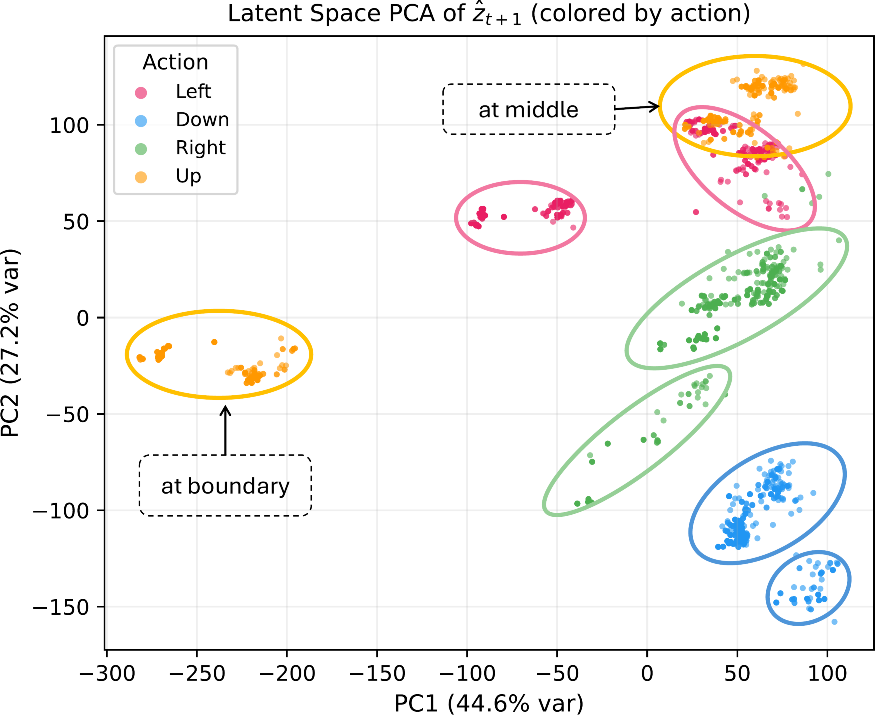
\includegraphics[width=0.72\linewidth]{results/figures/latent_pca_marked.pdf}
\caption{PCA of pooled $\hat{z}_{t+1}$ tokens colored by action (2000 test samples).
Distinct clusters per action direction confirm action-conditioned latent structure.
Each cluster further splits into two sub-clouds corresponding to boundary no-ops
(agent at wall) and effective transitions (agent moves).}
\label{fig:pca}
\end{figure}

% ── 7. Discussion ─────────────────────────────────────────────────────────────
\section{Discussion}

\paragraph{Emergent State-Action Context in the Latent Space.}
The bimodal clustering in Figure~\ref{fig:pca} reveals that $f_\theta$ has learned
to represent not just \emph{which} action was taken but also \emph{whether} it was
effective.
In FrozenLake, 24.7\% of test transitions are boundary no-ops where $o_t = o_{t+1}$.
For these, the latent predictor must output $\hat{z}_{t+1}$ that decodes to the
same observation as $o_t$, while for effective transitions it must predict a
shifted agent position.
The predictor implicitly learns this distinction, clustering no-op latents near an
``identity'' manifold shared across all four action directions, and effective-transition
latents in action-specific regions.

\paragraph{Rollout Stability.}
Per-step PSNR plateaus near 31.9\,dB after step 8 and never falls below the Stage\,0 proxy
(Figure~\ref{fig:drift}), a behavior we attribute to $\lambda\mathcal{L}_\text{embed}$
creating a basin of attraction that prevents runaway drift.
Without this term, Drift$_5$ increases 65\%.
The dec\_partial ablation achieves 49.6\,dB by jointly adapting the decoder during Stage\,2 ---
a degenerate result since freed output layers can memorize the rendering function
rather than learning a general world model; freezing the decoder is therefore an intentional
inductive bias, not a limitation.

\paragraph{Staged Training as Optimization Decomposition.}
End-to-end training from scratch fails catastrophically (9.45\,dB without Stage\,0),
because $g_\phi$ receives incoherent gradients before it has learned the visual domain.
Each stage reduces the search space: Stage\,0 establishes the visual prior,
Stage\,1 aligns the latent channel with the encoder manifold (cosine similarity $>$0.997),
and Stage\,2 grounds pixel-level predictions within the stabilized latent channel.
This decomposition is the primary reason a 5.8\,M parameter model can train
successfully from scratch on a single GPU in under 3 hours.

\paragraph{Why WM Look-Ahead Did Not Help Planning.}
\label{sec:discussion}
The tie at 5\% SR between VLM-only and VLM+WM traces to two compounding issues.
First, \emph{task mismatch}: the VLM was fine-tuned to output action words but is
implicitly asked to judge future states --- the lookahead filter can only discard
actions whose predicted frame elicits an explicit reversal, a rare signal.
Second, \emph{greedy myopia}: single-step look-ahead is equivalent to greedy search
in the WM's latent space, which can still walk into dead ends without backtracking.
Meaningful gains would require multi-step WM rollouts paired with a dedicated value
function, or a scoring function trained directly on (predicted frame, goal) pairs.

% ── 8. Conclusion ─────────────────────────────────────────────────────────────
\section{Conclusion}

We presented a three-stage training pipeline for learning action-conditioned
world models via structured latent token blocks.
On FrozenLake, our model achieves \MAINPSNR\,dB PSNR one-step and
Drift$_{10}$\,=\,\MAINDRIFTX\ over 10-step rollouts, outperforming all ablation
baselines.
A downstream evaluation pairs the WM with a fine-tuned Qwen2-VL-2B;
both VLM-only and VLM+WM reach \PLANVLMSR\ success rate, revealing that
high-fidelity prediction alone is insufficient for task improvement without
stronger search or a learned value function.
The key insight is that separating decoder adaptation (Stage\,0), latent format
stabilization (Stage\,1), and transition grounding (Stage\,2) substantially
eases optimization compared to end-to-end training from scratch.

\paragraph{Limitations.}
Compounding error causes quality degradation beyond 15 steps.
The planning evaluation exposes a gap between prediction quality and task utility:
single-step WM look-ahead does not improve over the VLM-alone baseline (both 5\%),
since greedy one-step search cannot recover from local dead ends and the reversal
filter is too weak to meaningfully redirect an already-confused policy.
The FrozenLake domain is also deterministic and visually simple; richer environments
(stochastic transitions, continuous actions) would stress-test the approach.
Future work includes multi-step WM rollouts with learned value functions,
scheduled sampling, and contrastive embedding objectives.

% ── References ────────────────────────────────────────────────────────────────
\bibliographystyle{plain}
{\small
\begin{thebibliography}{99}

\bibitem{hafner2019dream}
D.~Hafner et al.,
\emph{Dream to Control: Learning Behaviors by Latent Imagination},
ICLR 2020.

\bibitem{ha2018world}
D.~Ha and J.~Schmidhuber,
\emph{World Models},
NeurIPS 2018.

\bibitem{oh2015action}
J.~Oh et al.,
\emph{Action-Conditional Video Prediction using Deep Networks in Atari Games},
NeurIPS 2015.

\bibitem{hafner2020mastering}
D.~Hafner et al.,
\emph{Mastering Atari with Discrete World Models},
ICLR 2021.

\bibitem{hu2023gaia}
A.~Hu et al.,
\emph{GAIA-1: A Generative World Model for Autonomous Driving},
arXiv:2309.17080, 2023.

\bibitem{burchimudreamer}
M.~Burchi and R.~Timofte,
\emph{MuDreamer: Learning Predictive World Models without Reconstruction},
arXiv:2405.15083, 2024.

\bibitem{bruce2024genie}
J.~Bruce et al.,
\emph{Genie: Generative Interactive Environments},
ICML 2024.

\bibitem{cheng2025embodiedeval}
Z.~Cheng et al.,
\emph{EmbodiedEval: Evaluate Multimodal LLMs as Embodied Agents},
arXiv:2501.11858, 2025.

\bibitem{hu2025ewmbench}
Y.~Hu et al.,
\emph{EWMBench: Evaluating Scene, Motion, and Semantic Quality in Embodied World Models},
arXiv:2505.09694, 2025.

\bibitem{towers2024gymnasium}
M.~Towers et al.,
\emph{Gymnasium: A Standard Interface for Reinforcement Learning Environments},
arXiv:2407.17032, 2024.

\bibitem{wang2004ssim}
Z.~Wang et al.,
\emph{Image Quality Assessment: From Error Visibility to Structural Similarity},
IEEE Trans.\ Image Process., 2004.

\bibitem{wang2024qwen2vl}
P.~Wang et al.,
\emph{Qwen2-VL: Enhancing Vision-Language Model's Perception of the World at Any Resolution},
arXiv:2409.12191, 2024.

\end{thebibliography}
}

\end{document}
